%\documentclass[fleqn]{book}
\documentclass[11pt]{amsbook}

\usepackage[turkish]{babel}

%\usepackage{../HBSuerDemir}	% ------------------------
\usepackage{../Ceyhun}	% ------------------------
\usepackage{../amsTurkish}


\begin{document}

% ++++++++++++++++++++++++++++++++++++++
\hPage{192}
% ++++++++++++++++++++++++++++++++++++++
\begin{figure}
    \centering
    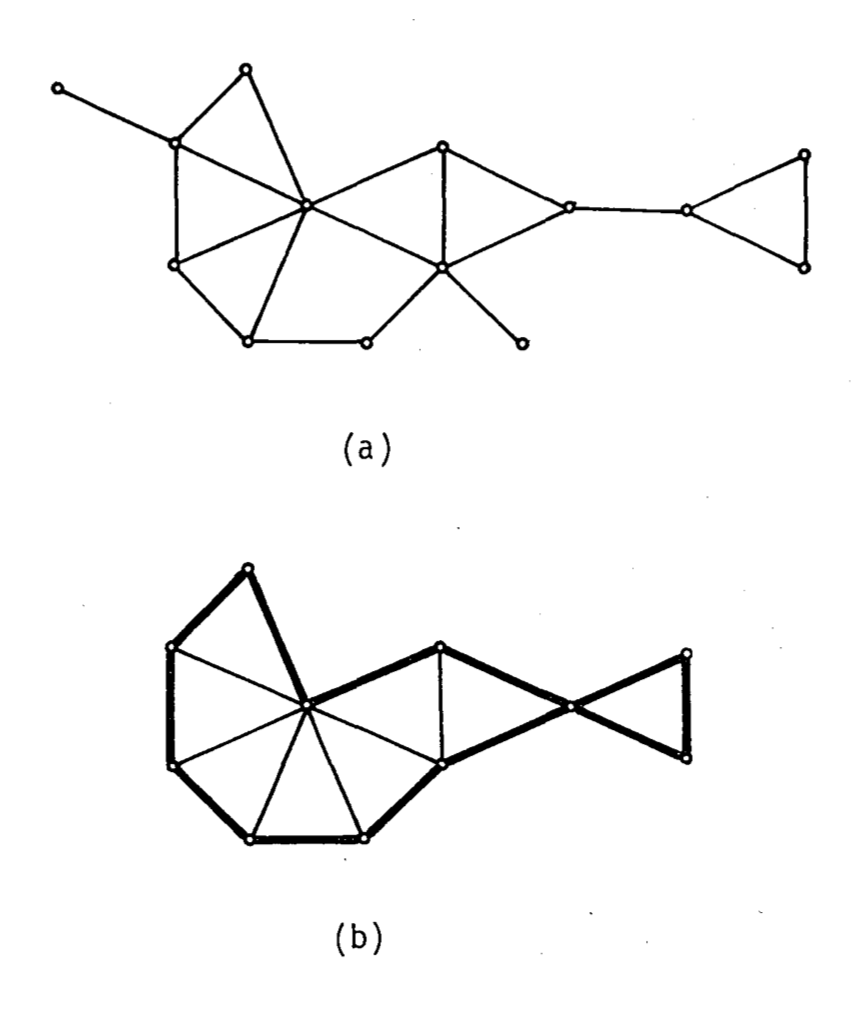
\includegraphics[width=0.8\textwidth]{images/Ceyhun-192-fig01.png}
    \caption{Çepersel çizge}
\end{figure}

\begin{theorem}

  Ç(d,a) nın çepersel olabilmesi için gerek ve yeter koşul, hiçbir altçizgesinin 
  $\theta_{1}$ ya da $\theta_{2} $
  çizgelerine kökteş olmamasıdır.
  
 \end{theorem}
\end{document}